\documentclass[12pt,fleqn]{article}\usepackage{../../common}
\begin{document}
Sonlu Öğeler Metotu (Finite Elements Method -FEM-) - Mittal

Alternatif Anlatım

Fonksiyonların İç Çarpımı (Inner Product)

Vektörlerden bildiğimiz çoğu tekniği fonksiyonlara uygulamak mümkündür [3].
Elimizde $f(x), g(x), ...$ reel değerli, $\alpha \le x \le \beta$ aralığında
tanımlı fonksiyonları olduğunu düşünelim, bu fonksiyonlar bir reel vektör uzayı
oluştururlar. Şimdi $(f,g)$ iç çarpımını düşünelim, ki bu çarpım tanımı

$$
(f,g) = \int _{\alpha}^{\beta} f(x) g(x) \ud x
$$

olsun. Üstteki bizim tanımımız tabii, başkaları ekler yapabilirler, mesela
bazıları iç çarpıma bir ağırlıklama fonksiyonu $w$ ekliyorlar, yani üstteki
entegralde $f,g$ ve $w$ çarpılıyor. Bizim dersimizin amaçları için biz
gördüğümüz tanımla yetineceğiz.

Üstteki entegral lineer. Simetrik olduğu bariz. Ayrıca kesin artı (positive
definite) özelliği de var.

Eldeki iç çarpım tanımıyla artık ``bir fonksiyonun uzunluğu'' bile
hesaplanabiliyor, aynen vektörlerin uzunluğunun hesaplanabildiği gibi.

$$
|| f || = \sqrt{ (f,f) } =
\sqrt{\int_{\alpha}^{\beta} f(x) f(x) \ud x } =
\sqrt{\int_{\alpha}^{\beta} [f(x)]^2 \ud x }
$$

Bu sayede birim fonksiyonlar bile yaratabilirim, mesela $f(x)$'i uzunluğu
$||f(x)||$ ile bölersem onu normalize etmiş olurum, yani uzunluğu bire inmiş
olur, $g$, $h$, vs ile bunu aynı şekilde gerçekleştirebilirim.

Tamlık (Completeness)

Bir $\alpha \le x \le \beta$ aralığında tanımlı fonksiyonlar kümesi $S$ olsun.
Ayrıca $y_0,y_1,..$ aynı $S$ kümesinde tanımlı birimdik (orthonormal)
fonksiyonlar olsun (yani her $y_i$ fonksiyonun birbiri ile iç çarpımı sıfır
sonucu verecek). Bu birimdik fonksiyonlar kümesine tam denir eğer herhangi bir
$f \in S$'i o baz fonksiyonların lineer kombinasyonu olarak yaklaşık şekilde
temsil edebiliyorsam. Yaklaşıklık derecesi benim tanımladığım $\epsilon > 0$ ile
ölçülecektir, ve kaç tane fonksiyonu kombine ettiğim de yine benim tarafımdan
tanımlı olacaktır. Yaklaşıklık

$$
|| f - (k_0 y_0 + k_1 y_1 + k_2 y_2 + ... + k_m y_m)  || < \epsilon
$$

ile ölçülebilir.

Not: Birimdiklik tamlık için şart değil, fakat birimdiklik bazı rahat işlemler
yapabilmemizi sağlar, o bakımdan tercih edilir.

Örnek

$-\pi \le x \le \pi$ arasında tanımlı bir $f(x)$ olsun. O zaman Fourier
fonksiyonları $1$, $\sin x$, $\cos x$, $\sin 2x$, $\cos 2x$, ... bir tam küme
oluştururlar. Çünkü $-\pi \le x \le \pi$ arasında bana verilen herhangi bir
fonksiyonu Fourier fonksiyonlarının bir kombinasyonu olarak temsil edebilirim,
ya da doğru terminoloji kullanmak gerekirse, onu bir ``Fourier Serisi'' olarak
temsil edebilirim. Görülen o her birimdik fonksiyonu $a_0$, $b_0$, $a_1$, $b_1$,
.. sabitleriyle çarpıp toplarım ve yaklaşık temsili yaparım, tabii katsayıların
ne olduğunu bulmam gerekir, doğru olanlarını bulunca $f$'yi iyi temsil etmiş
olurum. Seriyi uzattıkça, daha fazla Fourier terimi ekledikçe, $f$'ye daha da
yaklaşırım, benden beklenen $\epsilon$ yakınlığını böylece elde edebilirim. 
Mesela kabaca bir yaklaşıklık için 4-5 tane terim, çok iyi olması için
yüzlerce. 

Örnek

Herhangi bir kupsel polinomu temsil etmek bağlamında $1,x,x^2,x^3$ bir
tam küme oluşturur. Fakat bu küme yegane küme mi? Hayır. Mesela
$5$, $3+x$, $9 + 2x + 6x^2$, $5x + 20x^2$ kümesi de tamdır.

Tam küme öğelerinin bir özelliğine dikkat çekmek gerekir, onların birini
diğerlerinin lineer kombinasyonu olarak temsil etmek mümkün değildir.
Mesela $x^3$'u $1$, $x$, $x^2$'yi lineer olarak birleştirerek erisemem. 

Örnek

Bu örnekte tam olmayan bir kümeye bakalım. Mesela küpsel polinomları temsil
etmek için $1,x,x^3$ tam değildir, çünkü $x^2$ eksik. Mesela üstteki
$9 + 2x + 6x^2$ fonksiyonu.. onu eldeki bu baz ile temsil edemem çünkü
$x^2$ bazı yok. Evet $x^3$ var ama oradan ``aşağı inerek'' karesel temsil
yapmak mümkün değil, en azından benden istenen $\epsilon$ yakınlığında,
ve lineer kombinasyonlar kullanarak bunu yapmak mümkün değil.

Teori

$y_0,y_1,y_2,..$ fonksiyonları $S$ kümesi için, $\alpha \le x \le \beta$
aralığında tanımlı, tam, ve birimdik (bu sefer şart) bir küme olsun. O zaman
$f \in S$ bir sürekli fonksiyon ise ve her $y_m$'e dikgen ise bu demektir ki
$f$ muhakkak sıfırdır.

Mesela iki boyutta basit bir örnek üzerinde görelim; iki birimdik baz var, $x$
ve $y$ üzerinde kalın çizgi ile gösterdiğim, $i,j$ diyelim, şimdi bir $A$
vektörü düşünelim, bu vektör çizildiği haliyle tabii, birimdik $i,j$
kombinasyonu ile temsil edilebilir. Fakat şimdi düşünelim, eğer $A$
hem $i$'ye hem $j$'ye dikgen olsaydı, yani öyle bir vektör olsaydı ki
ne $x$ ne $y$ üzerinde hiçbir yansıması olmasaydı, bu $A$ sıfırdan başka
bir şey olamazdı, değil mi? Üstteki teorinin söylediği bundan ibaret. 

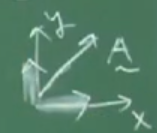
\includegraphics[width=10em]{compscieng_app45aerofem1_03.png}


Ağırlıklı Artıklar Metotu (Weighted Residual Method -WRM-)

Önceki derste iyi koşullu bir sistemi elde etmeyi gördük, bu kötü koşullu (ill
conditioned) olmanın tersi tabii. Bu derste WRM'yi kurmayı göreceğiz [1], ki bu
metot aslında kapsayıcı bir tarif, altında farklı hesap yöntemleri de
olabiliyor, WRM'nin kendisi hata kontrolünü nasıl yapacağımızı tarif ediyor.

Basit bir problemle başlayalım. Laplace formülü mesela, iki boyutu baz alalım,
ama birazdan göreceğimiz fikirler 1D ya da 3D için de geçerli. Problem bölgesi
(domain) $\Omega$ olsun onun sınırları $\Gamma$, 

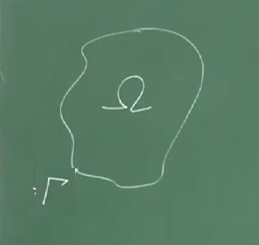
\includegraphics[width=15em]{compscieng_app45aerofem1_01.png}

İlgilendiğimiz alan (field) $T(x,y)$, bu reel değerli bir fonksiyon, ve
kurduğumuz sistem için bu fonksiyonun şu şartlara tabi olmasını istiyoruz,

$$
\nabla^2 T = 0 \quad \Omega \textrm{ üzerinde } 
$$

$$
\Gamma \textrm{ için } T = T_0
$$

Bu tür problemlere Drichlet problemleri deniyor.

Üstteki şartları yerine getiren bir $T(x,y)$ çözümü bulmak istiyoruz. O zaman
ilk akla gelen nedir? Diferansiyel denklemi alıyorum ve $\Omega$ içindeki tüm
noktalar için çözmeye uğraşıyorum. Fakat bu kolay değil. Ayrıca $\Omega$'daki
eşitlik $\Gamma$ sınırında geçerli değil, ikinci şart sebebiyle. Bu arada
matematiksel olarak çözüm nedir? $\Omega$'daki sonsuz tane nokta için geçerli
olan şeydir. Buna kesin çözüm (exact solution) deniyor. 

Fakat bu çözümü bulmak mümkün değilse, ya da yaklaşık bir çözüm de yeterli
oluyorsa o zaman yaklaşık yöntemler kullanabilirim.. $\nabla^2 T = 0 $ eşitliği
$\Omega$'daki her nokta için, her $\Gamma$ sınır şartında değil belli seçilmiş
noktalarda olsun diyebilirim.

Ama ``belli noktalarda'' deyince de iş bitmiyor, o seçilmiş noktalarda kesin
çözüm mü yapsam, yoksa o noktalarda da yaklaşık çözüm yapsam? Ya da tüm
noktalarda yaklaşık çözüm üzerinden bir hata hesaplayıp, tüm seçilmiş noktalarla
hesaplanan ortalama bir hatanın sıfır olması için mi uğraşsam?

Şöyle bir yöntem deneyelim; elimizde / verili belli bir baz fonksiyon ``sınıfı''
olsun, bu fonksiyonlar Fourier bazı $\sin$, $\cos$ olabilir, ya da Chebisev
polinomları olabilir. Bu ``test'', baz fonksiyonları $T_i(x,y)$ içinde,
$i=1,2,...,N$, ve nihai $T$'yi

$$
T = T_0 + \sum _{i=1}^{N} c_i T_i(x,y)
$$

ile hesaplayayım, $c_i$'ler başta bilmediğim katsayı değerleri olsun. Bilinen /
verili test fonksiyonları üzerinden doğru $c_i$'leri bulursam bu beni gerçek
fonksiyon $T$'ye yaklaştırır. Üstteki toplamda $T_0$ terimi özellikle o şekilde
formüle dahil edildi, $T_i$ toplamının sınırda sıfır olmasını ayarlayabilirsem,
$T=T_0$ şartını otomatik olarak tatmin etmiş olurum.

$N$ sayısına dikkat, gerçek fonksiyonu aşağı yukarı temsil etmek istesem $N$'yi
az tutardım, birkaç tane temel fonksiyon birleşimi.. Ama $N$'i arttırarak, hatta
sonsuza yaklaştığımızda gerçek fonksiyona tıpatıp eşit olacağımızı
bekleyebilirdik, o zaman $N$ sayısı bir anlamda yaklaşıklamanın kalitesini
kontrol edecektir. $N$ arttıkça hata azalır, yaklaşıklama gerçeğe yaklaşır.
Bir ödünleşim (trade-off) durumu var muhakkak, çok büyük $N$ hesaplaması zor
olan bir sistem ortaya çıkartabilir, vs.

Bu bizi hata tanımına getiriyor. Onu gerçek ve yaklaşık değerler arasındaki
fark, ``artık'' (residual) üzerinden tanımlayacağız, artık $R$,

$$
R(c_i,x,y) = \nabla^2 T
$$

Bu kadar basit. Niye artığı direk $\nabla^2 T$'e eşitlemek yeterli? Çünkü ana
formüle bakarsak $\nabla^2 T$ ideal durumda sıfır olmalı değil mi?  Ama
yaklaşıklama mükemmel olmadığı için sıfırdan farklı (fakat umuyoruz ki ona
yakın) değerler döndürecektir, o zaman bu değeri alıp direk hata / artık değeri
olarak kullanabiliriz. O zaman

$$
R(c_i,x,y) = T_0 + \sum _{i=1}^{N} c_i T_i(x,y)
$$

diyelim. Üstteki denklem bana her veri noktası, belli bir $x,y$ için olan hatayı
verir. Sınır koşulunu denklem doğal olarak karşıladığı için orada zaten hata
yok. Yani tanım itibariyle sınırda hata sıfır, ve sınırlar içinde muhtemel
olarak sıfır olmayan bir değerde.

Şimdi $c_i$'lerin bulunmasına gelelim, yaklaşık temsil onlar üzerinden mümkün
olacak. $N$ tane $c_i$ bilinmiyor o zaman bir şekilde $N$ tane denklem üretmem
lazım, ki onları çözerek bilinmeyenleri elde edeyim. WRM burada devreye giriyor.

Ağırlıklı artıklar dedik, ağırlıklardan da (dikkat $c_i$ katsayılarından, ve
test fonksiyonlarından farklı bu) da $N$ tane var, $N$ tane fonksiyon. Onları
$j$ ile indisleyebiliriz, $w_j$, $j=1,...,N$. Artıkları şöyle ağırlıklıyoruz,

$$
\int_\Omega w_j R \ud \Omega
$$

Biraz önce söylediğimiz artığın sıfır olma hedefini biraz genişletip
ağırlıklanmış artığın sıfır olması haline getiriyoruz. O zaman $N$ tane denklemi
şöyle üretiriz,

$$
j=1,\quad
\int_\Omega w_1 (x,y) \left[
  \nabla^2 T_0 + \sum _{i=1}^{N} c_i \nabla^2 T_i(x,y) 
  \right] \ud \Omega
$$

$$
j=2,\quad
\int_\Omega w_2 (x,y) \left[
  \nabla^2 T_0 + \sum _{i=1}^{N} c_i \nabla^2 T_i(x,y) 
  \right] \ud \Omega
$$

$$
\vdots
$$

$$
j=N,\quad
\int_\Omega w_N (x,y) \left[
  \nabla^2 T_0 + \sum _{i=1}^{N} c_i \nabla^2 T_i(x,y) 
  \right] \ud \Omega
$$

Böylece $N$ tane bilinmeyen için $N$ tane formül elde ettim, ve bu şekilde
çözümü yapabilirim.

$w_j$'ler ne yapıyor? Başta hataların ortalamasından bahsetmiştik hatırlarsak,
her $w_j$ bir nevi ortalamadır, ama her $j$ için farklı bir ortalama şekli
seçebiliriz, mesela alttaki resimde

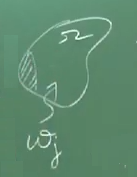
\includegraphics[width=10em]{compscieng_app45aerofem1_02.png}

karalanmış kısma daha fazla ağırlık ver diyebiliriz, vs. Genel anlamda
hatırlarsak üç sayı A,B,C ortalaması demek aslında her sayının 1/3 ``ağırlığı''
ile çarpılıp, toplanması ve sonucun 3'e bölünmesi demektir. Bu ağırlıkları
değiştirebiliriz, o zaman farklı bir ortalama elde ederiz, mesela 1/2, 1/4, 1/4
kullansam A'ya daha fazla ağırlık vermiş olurdum.

Bu açıdan bakınca üstte üretilen her denklem belli bir artık formülünün
farklı şekillerde ağırlıklanması sonucu elde edilen denklemlerdir.

Galerkin Metotu

Bu metot FEM'in temelini oluşturur [2], 1915, 1913'te Galerkin, Bubnov
tarafından ayrı ayrı keşfedilmiştir. Galerkin metotunun özü şu basit önermeden
ibaret, daha önce gördüğümüz ağırlıklı artıklar metotunda Galerkin metotu der ki
$w_j = T_j$, yani ağırlık fonksiyonu test fonksiyonu ile aynı olsun. Ayrica
hatirlarsak $T_j$'lerin bir tam kume olusturmasi gerekiyor, o zaman $w_j$'lerin
de tam kume olusturmasi gerekiyor. Bu durumda agirlikli artiklar metotu bizi su
noktaya getirir,

$$
(w_j,R) = 0
$$

Yani $R$ her $w_j$'e dikgen, bu daha önceki dikgenlik teorisini hatırlatmalı
bize, eğer $R$ her birimdik baz fonksiyonuna dik ise, kendisi sıfırdan başka bir
şey olamaz. Bu çok kuvvetli bir sonuç. $R$ hatasının tam kümedeki her fonksiyon
ile iç çarpımının sıfır olma şartına bakıyoruz.. bu tür bir ilişkinin bize
ileride faydalı olacağını görmek zor değil, dikgenlikten direk $R$'nin sıfır
olmasına atlayabilmiş oluyoruz, bunu lineer cebirsel işlemlerimizde
kullanabiliriz.

Kaynaklar

[1] Mittal, {\em FEM for Fluid Dynamics, Lecture 07 Part A, Method of Weighted Residuals, IIT Kanpur},
    \url{https://www.youtube.com/channel/UCWheqBdP45xBVp_Eqi1eltQ/videos}

[2] Mittal, {\em FEM for Fluid Dynamics, Lecture 07 Part B, IIT Kanpur},
    \url{https://www.youtube.com/channel/UCWheqBdP45xBVp_Eqi1eltQ/videos}

[3] Mittal, {\em FEM for Fluid Dynamics, Lecture 05 Part C, Inner Product for functions,Orthogonality,Completeness, IIT Kanpur},
    \url{https://www.youtube.com/channel/UCWheqBdP45xBVp_Eqi1eltQ/videos}


    
\end{document}





